\documentclass[11pt,a4paper]{moderncv}
\moderncvstyle{banking}
\moderncvcolor{blue}

\usepackage[utf8]{inputenc}
\usepackage[spanish,es-lcroman,es-notilde]{babel}
\usepackage[scale=0.75, top=2cm, bottom=3cm]{geometry}
\usepackage{import,lastpage,fontawesome,xpatch}
\usepackage[absolute,overlay]{textpos}
\renewcommand*{\titlefont}{\fontsize{21}{25}\mdseries\upshape}

\AtEndPreamble{
    \hypersetup{
        pdfauthor     = Federico del Mazo,
        pdftitle      = Curriculum Vitae - Federico del Mazo,
        pdfsubject    = Curriculum Vitae - Federico del Mazo,
    }
}

\makeatletter
\xpatchcmd{\makehead}{\titlestyle{~|~\@title}}{\par\vskip1ex\titlestyle{\@title}}{}{}
\makeatother

\name{Federico}{del Mazo}
\title{Curriculum Vitae}
\extrainfo{Beruti 545, Ramos Mejía (1704)}
\address{21 años, estudiante de ingeniería en informática}{}{}
\phone[mobile]{11 6110 1997}
\phone[fixed]{4656 4494}
\email{delMazoFederico@gmail.com}
\extrainfo{\faLinkedin \vspace{0.4mm} delMazoFederico • \faGithub \vspace{0.4mm} FdelMazo}

\begin{document}

\begin{picture}(0,0)
\put(-30,-110){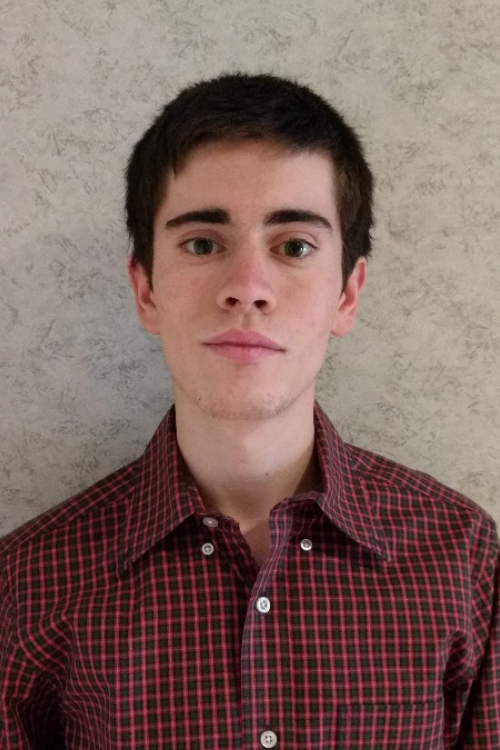
\includegraphics[scale=0.20]{fotoCV}}
\end{picture}

\makecvtitle
\small{Joven estudiante en busca de iniciarse en el mercado laboral con el objetivo de enriquecer sus conocimientos y desarrollarse en sus primeras experiencias profesionales.}

\section{Experiencia laboral}
\vspace{6pt}
\cventry{Abril 2018--Actualidad}{Desarrollador full stack}{Raiconet}{}{}{}

\section{Experiencia laboral no rentada}
\vspace{6pt}
\cventry{Agosto 2017--Actualidad}{Ayudante de Algoritmos y Programación II - Curso Wachenhauzer}{Universidad de Buenos Aires, Facultad de Ingeniería}{}{}{}

%\section{Materias aprobadas en la Facultad de Ingeniería}
%\vspace{6pt}
%\cventry{12/12/01}{95-4264}{Algoritmos y Programación I (75.40)}{Calificación: 8}{}{}
%\vspace{6pt}
%\cventry{16/02/17}{62-2705}{Física I (62.01)}{Calificación: 4}{}{}
%\vspace{6pt}
%\cventry{21/02/17}{61-0002637}{Analisis Matemático II (61.03)}{Calificación: 6}{}{}
%\vspace{6pt}
%\cventry{03/07/17}{95-4712}{Algoritmos y Programación II (75.41)}{Calificación: 9}{}{}
%\vspace{6pt}
%\cventry{10/08/17}{63-0002187}{Química (63.01)}{Calificación: 5}{}{}
%\vspace{6pt}
%\cventry{18/12/17}{95-5174}{Algoritmos y Programación III (75.07)}{Calificación: 6}{}{}


\section{Educación}
\vspace{6pt}
\cventry{2015--Actualidad}{Estudiante de Ingeniería en Informática}{Universidad de Buenos Aires, Facultad de Ingeniería}{}{}{}
\vspace{6pt}
\cventry{2009--2014}{Bachiller Bilingüe en Economía y Administración}{Colegio Ward}{}{}{\textit{Promedio general 8.29}} 
\vspace{6pt}
\cventry{2012--2013}{International General Certificate of Secondary Education (IGCSE)}{University of Cambridge}{}{}{\textit{Passed with Merit}}
%     Environtmental Management B
%     Geography B
%     First Language Spanish D
%     Economics B
%     Mathematics B
%     Business Studies C
%     First language english D
\vspace{6pt}
\cventry{2011}{First Certificate in English}{University of Cambridge}{}{}{\textit{Grade C}}
% Cambridge ESOL Level 1 Certificate in ESOL International
% General Knowledge Business Competition - Instituto Tecnológico de Buenos Aires - Carrera de Licenciatura en administracion y sistemas

\section{Conocimientos específicos}
\vspace{2pt}
\begin{itemize}
\vspace{2pt}
\item \textbf{Lenguajes de programación:} C, Python, Java, JavaScript, SmallTalk, Lua.
\vspace{2pt}
\item \textbf{Otros lenguajes:} SQL, TeX, HTML, CSS, UML.
\vspace{2pt}
\item \textbf{Otros:} jQuery, Bootstrap, Groovy, Grails.
\vspace{2pt}
\end{itemize}

\section{Intereses y actividades extracurriculares}
\vspace{6pt}
\begin{itemize}
\item \textbf{Programación} Todos mis proyectos personales (videojuegos, programas) pueden verse en mi perfil de Github.

\vspace{4pt}
\item \textbf{Cine} Desde siempre tengo una pasión por el cine y asistí a diversos talleres y cursos:
\begin{itemize}
\item{Jornada IV de Antropología e Imagen - Facultad de Filosofia y Letras de la UBA}
\item{Introducción al septimo arte, por Sebastián de Caro - Universidad CAECE}
\item{Realización cinematográfica, por Mariano Swi - CC Matienzo}
\end{itemize}

\vspace{4pt}
\item \textbf{Deportes} Entre los 10 y 17 años me desempeñé en handball en el equipo del Colegio Ward, saliendo campeón y subcampeón en distintas competencias de la Federación Metropolitana de Balonmano.

\vspace{4pt}
\item \textbf{Música} Entre los 12 y 18 años participé en la Banda del Colegio Ward tocando la trompeta y el piano. Con esta fuí a diversas convenciones musicales de Argentina.

\end{itemize}
\fancyhead{}
\fancyhead[R]{\color{gray}Federico del Mazo}
\fancyfoot{}
\fancyfoot[R]{\color{gray}\textit{Abril 2018 \\ \thepage/\pageref*{LastPage}}}

\end{document}
